\documentclass{beamer}
\usepackage[cp1251]{inputenc}
%\usepackage[russian]{babel}
\usepackage{amsmath,mathrsfs,mathtext}
\usepackage{graphicx, epsfig}
\usetheme{Warsaw}%{Singapore}%{Warsaw}%{Warsaw}%{Darmstadt}
\usecolortheme{sidebartab}
\definecolor{beamer@blendedblue}{RGB}{15,120,80}
%----------------------------------------------------------------------------------------------------------
\title[\hbox to 56mm{Spherical convolutions  \hfill\insertframenumber\,/\,\inserttotalframenumber}]
{Quality prediction of proteins models with spherical convolutions on three-dimensional graphs}
\author[N.\,V.~Pavlichenko]{Nikita Pavlichenko}
\institute{Moscow Institute of Physics and Technology}
\date{\footnotesize{
\par\emph{Course:} My first scientific paper\par Group 793, 2020
\par\emph{Consultants:} I. Igashov, S. Grudinin
\date{qq}
}}
%----------------------------------------------------------------------------------------------------------
\begin{document}
%----------------------------------------------------------------------------------------------------------
\begin{frame}
%\thispagestyle{empty}
\titlepage
\end{frame}
%-----------------------------------------------------------------------------------------------------
\begin{frame}{Goal of research}
    \begin{block}{Goals}
        \begin{itemize}
            \item Develop the new type of convolution operations on three-dimensional graphs
            \item Apply this method to Protein Quality Assessment problem
        \end{itemize}
        \end{block}
\end{frame}
%----------------------------------------------------------------------------------------------------------
\begin{frame}{Problem statement}
    \begin{block}{Problem statement}
    \begin{itemize}
        \item Protein can be represented as a graph - a chain of amino acids
        \item Its properties are determined by its folding
        \item We have lots of folding models and want to choise the best
        \item We need to predict quality of these models - regression problem on graph
        \item MSE seems the most suitable loss function
    \end{itemize}
    \end{block}
\end{frame}
%----------------------------------------------------------------------------------------------------------
\begin{frame}{Solution}
    \begin{block}{Graph Convolutional Networks}
        \begin{itemize}
            \item A very common method is Graph Convolutional Network
            \item $l$-th layer can be represented as $H^{(l)} = AH^{(l-1)}W^{(l)}$, where $A$ is the adjacency matrix, $W^{(l)}$ is weights matrix
        \end{itemize}
    \end{block}
    \begin{block}{Props and Cons}
        \begin{itemize}
            \item It was successfully applied for PQA before
            \item It does not capture a local protein structure
        \end{itemize}
    \end{block}
\end{frame}

\begin{frame}{Solution}
    \begin{block}{Spherical convolutions}
        \begin{itemize}
            \item Amino acids are connected one by another so we can define a local coordinate system for every amino acid
            \item So, let's project it's neighbors onto a unit sphere.
            \item Conider a function of spherical coordinates. It can be expaned as a series of spherical harmonics.
            \item $f(\phi, \psi) = \sum_{l = 0}^{\infty} \sum_{m=-l}^{m=l}f_l^m Y_l^m(\phi, \psi)$
            \item Leave only a few coeficients and write it in a matrix view
            \item $f(\Omega) \approx f_W(\Omega) = \sum_{l=0}^{L}\sum_m \boldsymbol{W}_l^m Y_l^m(\Omega)$
            \item Now we can introduce Spherical Convolution operation
            \item $f_W \circ v_i = \sum_{v_j \in \mathcal{N}(v_i)} f_W(\Omega_i^j)x(v_i)$
        \end{itemize}
    \end{block}
\end{frame}
% , $A$ - adjcency matrix, $W^{(l)}$ - weights, $H^(l-1)$ - output of $l-1$-th layer
%----------------------------------------------------------------------------------------------------------
\begin{frame}{Solution}
    \begin{block}{Spherical Convolutional Network}
        \begin{itemize}
            \item Spherical convolution layer: $\boldsymbol{X} \longrightarrow \boldsymbol{X}' = \sigma(f_W \circ \boldsymbol{X}) = \sigma\left(\sum_{l,m}Y_l^m(\boldsymbol{A}_\Omega)\boldsymbol{X}\boldsymbol{W}_l^m\right)$
            \item Learn $\boldsymbol{W}_l^m$ matrices using Adam optimizer
        \end{itemize}
    \end{block}
   %\includegraphics[width=0.7\textwidth]{fig/ErrorFunction}
\end{frame}

\begin{frame}{Computational experiment}
    \begin{block}{Dataset}
        \begin{itemize}
            \item We use CASP competition data. CASP8-CASP11 as a train sample and CASP12 as a testing sample.
            \item Spherical harmonics are precalculated: we use an order of 5 and it takes 60GB of HDD
        \end{itemize}
    \end{block}
    \begin{block}{Baseline}
        \begin{itemize}
            \item 8 GCN layers with 4 linear layers in the beggining as an encoder and 5 linear layers in the end is the best setup for GCN
            \item Learn on CPU since the loading from HDD is a bottleneck
        \end{itemize}
    \end{block}
    
    
   %\includegraphics[width=0.7\textwidth]{fig/ErrorFunction}
\end{frame}
%----------------------------------------------------------------------------------------------------------
\begin{frame}{Computational experiment}
    \begin{block}{Algorithm}
        \begin{itemize}
            \item Optimal architecture is 5 spherical convolution layers
            \item All code is written in PyTorch
            \item Learn on GPU in 4 parallel subprocesses
        \end{itemize}
    \end{block}
    \begin{block}{Results}
        \begin{itemize}
            \item The common choice for a quality metric is Pearson correlation between ground truth and predictions
            \item The best achieved result for GCN is $0.57$ comaring with $0.77$ with spherical convolutions
        \end{itemize}
    \end{block}
\end{frame}
\begin{frame}{Computational experiment}
    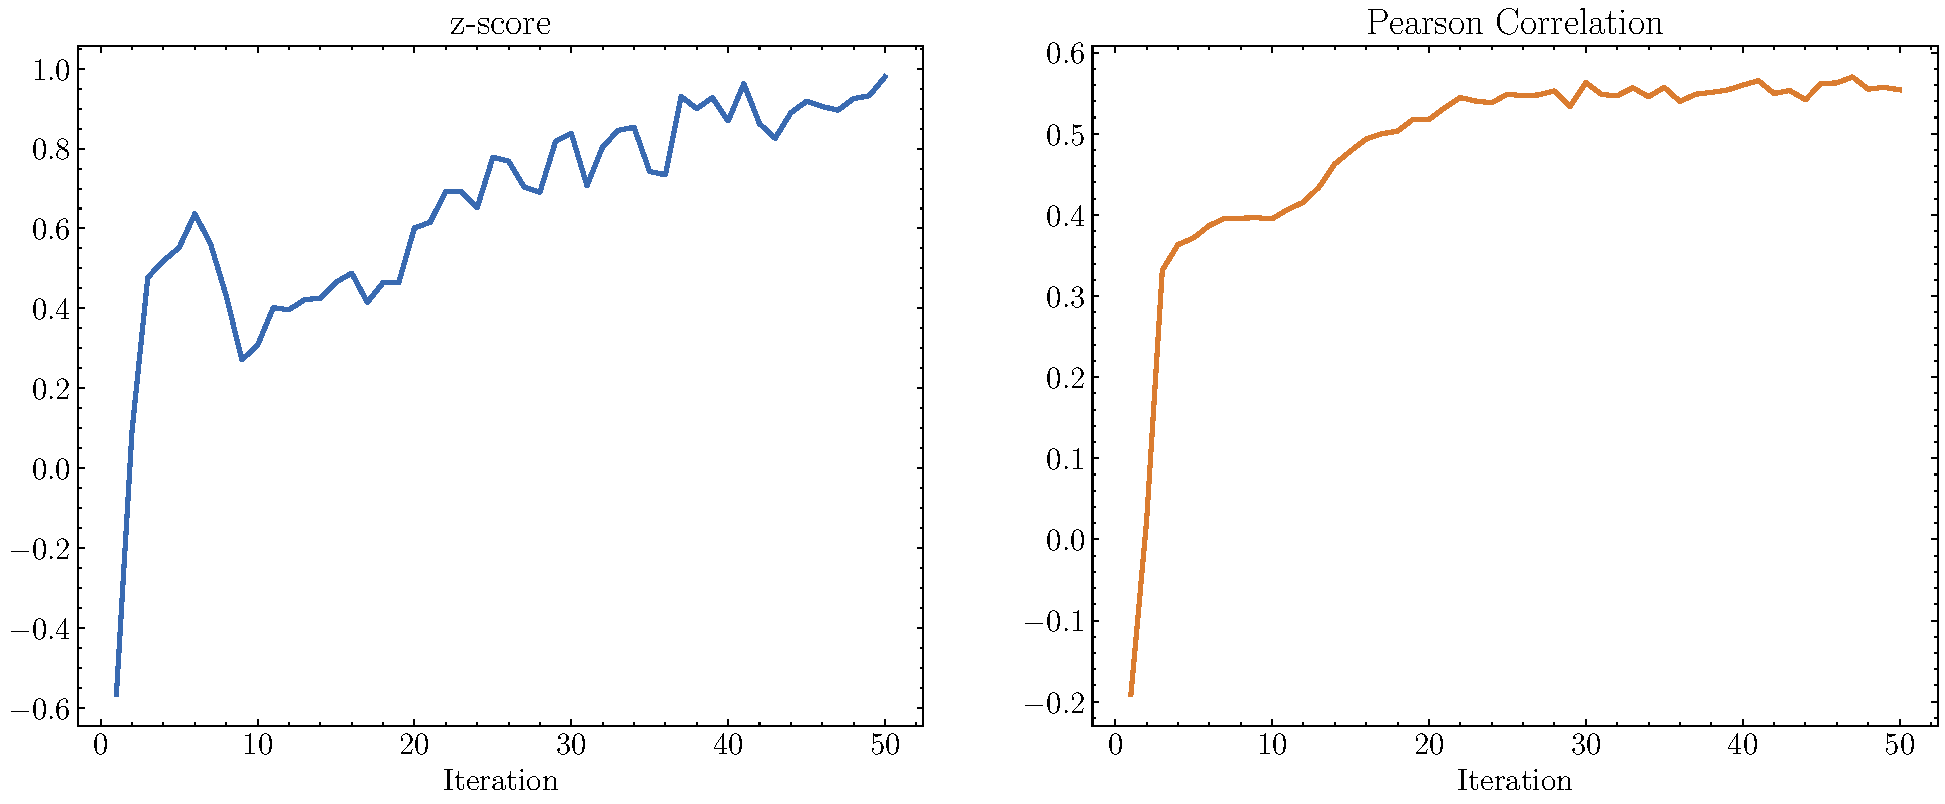
\includegraphics[width=1.0\textwidth]{img/z_score_casp12.pdf}
   %\includegraphics[width=0.7\textwidth]{fig/ErrorFunction}
\end{frame}
\begin{frame}{Computational experiment}
    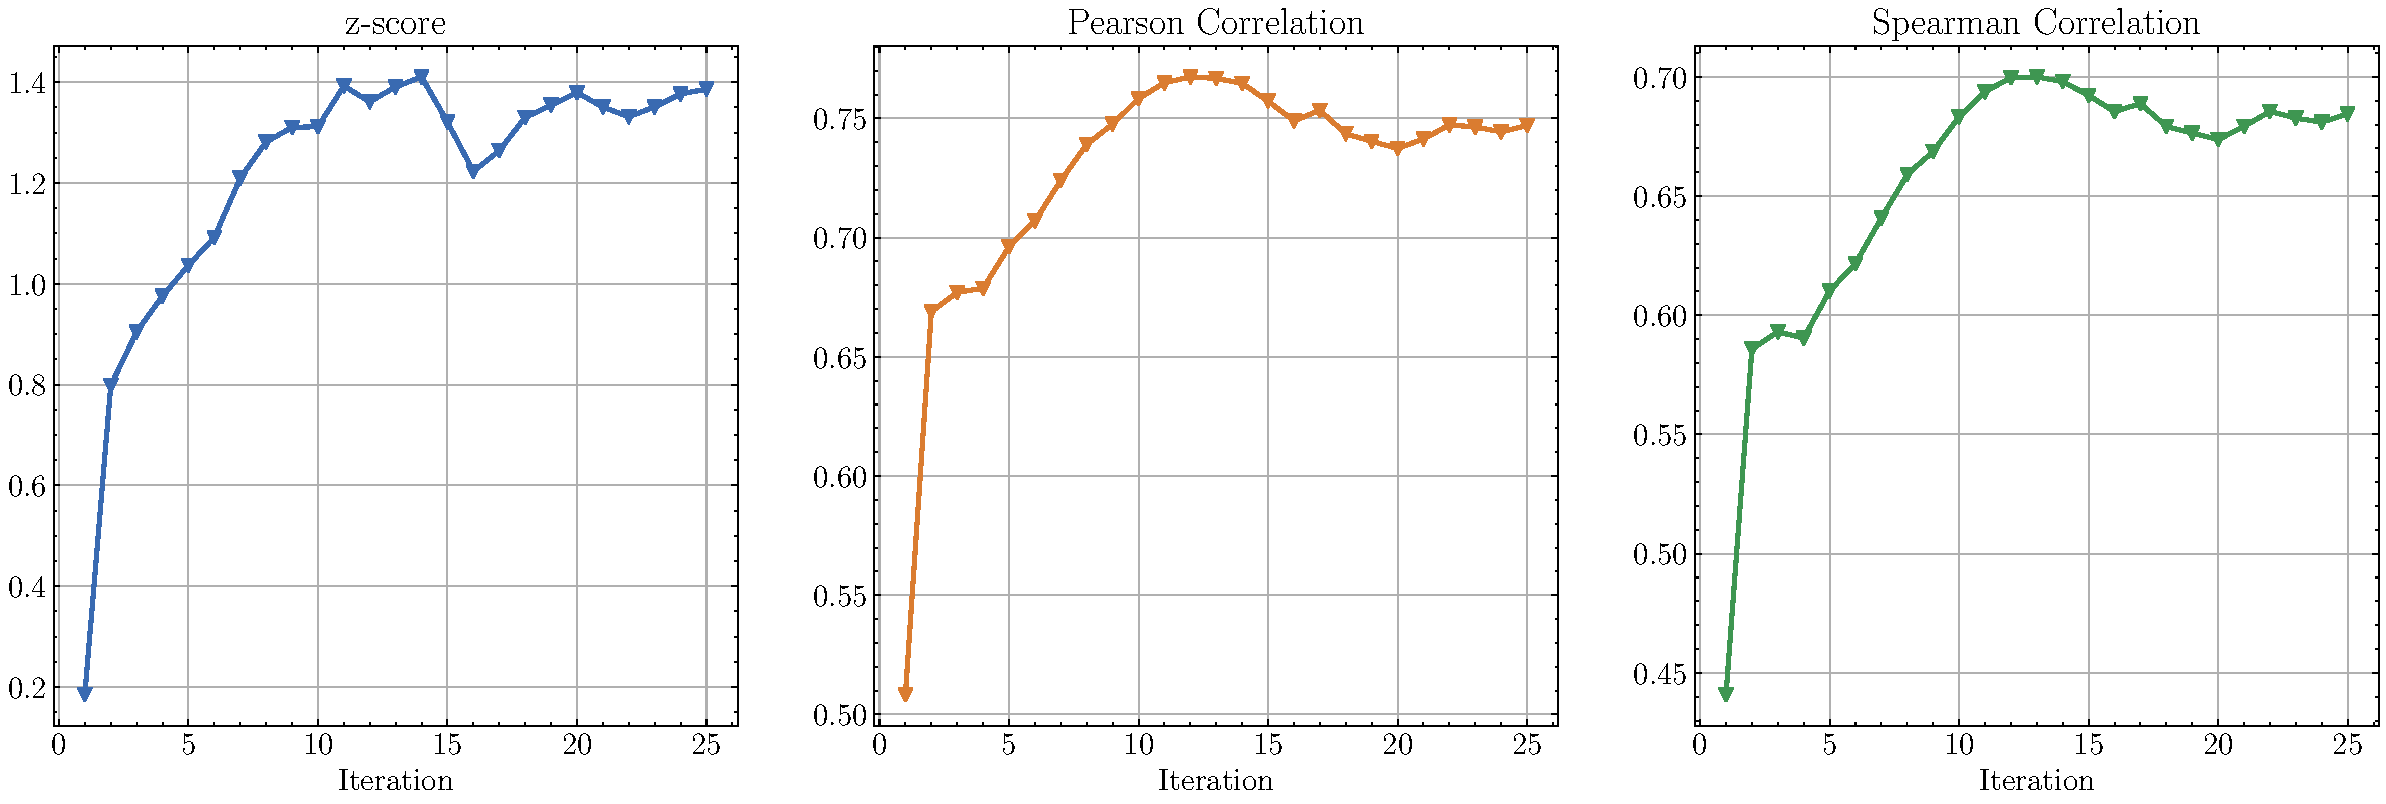
\includegraphics[width=1.0\textwidth]{img/z_score_casp12_sh.pdf}
   %\includegraphics[width=0.7\textwidth]{fig/ErrorFunction}
\end{frame}
\begin{frame}{Conclusion}
        \begin{itemize}
            \item For the first time we introduced spherical convolution operation
            \item It has shown a significant improvement in Protein Quality Assessment
            \item It potentially has a huge space for improvements e.g. variational autoencoders
        \end{itemize}
\end{frame}
%----------------------------------------------------------------------------------------------------------
\end{document} 
